% Created 2024-10-16 śro 21:35
% Intended LaTeX compiler: pdflatex
\documentclass[../../main.tex]{subfiles}

% \usepackage[a4paper, margin=3cm]{geometry}
% \usepackage{amssymb} // not working

\usepackage[T1]{fontenc}
\usepackage[utf8]{inputenc}
\usepackage{graphicx}
\usepackage{longtable}
\usepackage{wrapfig}
\usepackage{rotating}
\usepackage[normalem]{ulem}
\usepackage{amsmath}
\usepackage{capt-of}
\usepackage{hyperref}
\usepackage{siunitx}
\usepackage{float}
\usepackage[polish]{babel}

\graphicspath{{../}}
\author{Wojciech Paderewski}
\date{\today}
\title{ESP32}
\hypersetup{
 pdfauthor={Wojciech Paderewski},
 pdftitle={LDO},
 pdfkeywords={},
 pdfsubject={},
 pdflang={Polish}}

\begin{document}
ESP32-S3 wymaga jedynie dodania przycisków do resetowania i wprowadzenia w tryb programowania.
Dodano więc 2 przyciski, jeden do pinu EN (Enable) a drugi do pinu IO0, który jest pinem programowania,
każdy z przycisków ma dodatkowo podłączony kondensator ceramiczny o pojemności 100 nF, by zminimalizować zakłócenia oraz
rezystor podciągający o wartości 10 k$\Omega$.

Dodano, również kondensator odsprzęgający 100 nF na zasilanie ESP32-S3. W związku z tym, że większość pinów ESP32-S3 może 
pełnić dowolne funkcje, istniała duża dowolność w podłączeniu pinów, co pozwoliło na łatwiejsze rysowanie ścieżek na płytce drukowanej.
Schemat podłączenia ESP32-S3 przedstawiono na rysunku \ref{fig:esp32}.

\begin{figure}[H]
    \centering
    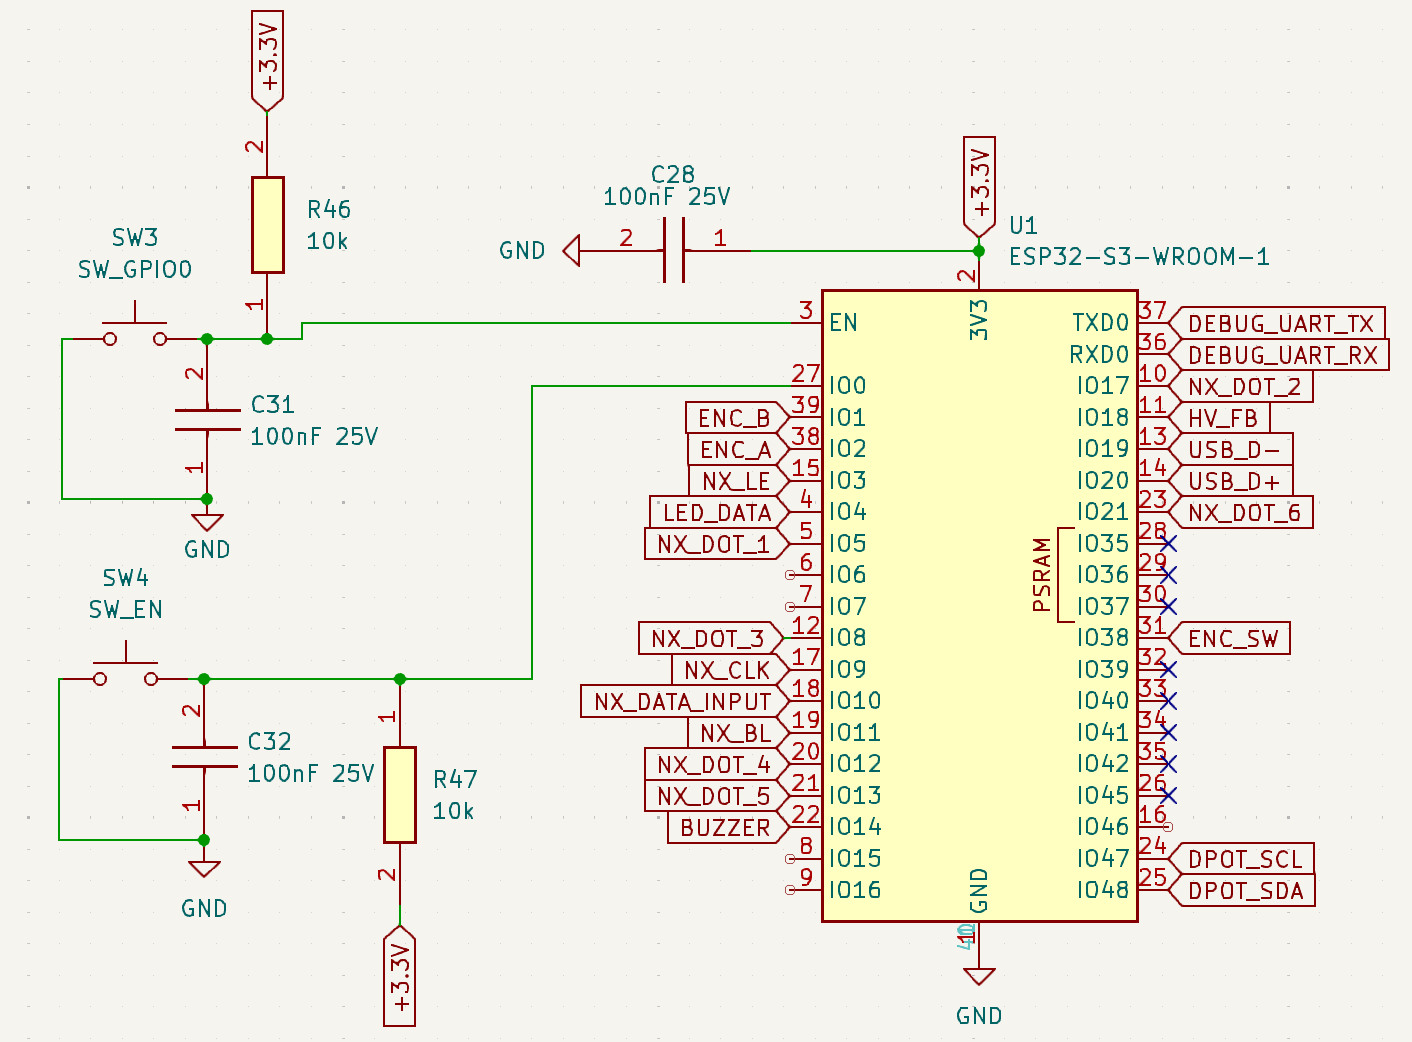
\includegraphics[width=0.8\textwidth]{ESP.png}
    \caption{Schemat podłączenia ESP32-S3}
    \label{fig:esp32}
\end{figure}

\end{document}
